\chapter{Theoretical Background}
\label{ch:Background}
In this chapter we define the necessary background for understanding PGExplainer as well as the follow-up work regarding its application on an ML solver for SAT. We start by giving an introduction to DL in Section \ref{sec:deep_learning}, including a specific architecture and regularization techniques. In Section \ref{sec:graph_theory} we define the necessary graph theory, including bipartite graphs and random graphs. To understand the motivation behind the objective of PGExplainer we outline the relevant concepts of information theory, namely entropy, cross-entropy and mutual information, in Section \ref{sec:information_theory}. Since the explainer model operates on Graph Neural networks, we introduce the historically relevant GNN model by Scarselli et al. ~\cite{4700287} in Section \ref{sec:gnns}, as well as three succeeding models. Lastly, in Section \ref{sec:SAT} we describe SAT as the problem that motivates this work.

\section{Deep Learning}
\label{sec:deep_learning}
In this chapter we introduce DL in the context of ML and their concepts required for this work. The definitions in this chapter loosely follow Goodfellow et al.~\cite{Goodfellow-et-al-2016}.

ML algorithms generally learn to perform certain tasks from data that can broadly be divided into supervised and unsupervised learning. In this work, we focus on supervised learning, meaning that the algorithm learns from a dataset containing both features and labels or targets that the algorithm is supposed to predict. In other words, the algorithm learns from a training set of input examples, defined as vectors $\mathbf{x} \in \mathbb{R}^d$, with entries $x_i$ denoting features, and output examples $y$. Its goal is to be able to associate unseen inputs from a set of test data, coming from the same distribution as the training data, with some target output.

This process estimates the generalization error of the learner after the training is complete. 
Common supervised ML tasks include classification, assigning an input to one of $k$ categories, and regression, where the program shall predict a numeric value given some input. \bigskip

DL entails expanding the size of the model used in our algorithm to allow for representations of functions with increasing complexity. This enables many human-solvable tasks that consist of mapping an input vector to an output vector to be performed with DL, given sufficiently large models and datasets. Most notably, Krizhevsky et al.~\cite{krizhevsky2012imagenet} achieved record-breaking results by using a large, deep convolutional network for image classification.

However, increasing the size of a model comes with new challenges. Since models become more complex with increasing number of layers, subnetworks and parameters, they are commonly treated as a "black box", as it is difficult to explain their decision-making process \cite{noor2024survey}. Thus, the need for methods that can explain and interpret such models arises. Furthermore, the increasing number of parameters directly raises the computational complexity, resulting in longer training times and higher hardware requirements. This may also impose limitations when deploying the model on low-resourced end-devices. \bigskip

In many cases DL involves optimizing an objective function that guides the model, usually by minimizing $f(x)$. This objective function is also referred to as loss function in the context of minimization. %We denote $x^*=\text{arg min} f(x)$.

To minimize a function $y = f(x)$, where $y,x \in \mathbb{R}$, we make use of the derivative $f'(x)$ that tells us how to change $x$ in order to get an improvement in $y$. We can reduce $f(x)$ by moving $x$ in the direction opposite of the sign of its derivative, since $f(x-\epsilon \text{ sign}(f'(x))) < f(x)$ for small enough $\epsilon$. Since we usually want to minimize a function with multiple inputs, we let $\mathbf{x} \in \mathbb{R}^n$ be a vector with $n$ elements. The partial derivative $\frac{\partial}{\partial x_i}f(\mathbf{x})$ is utilized, telling us how $f$ changes when only $x_i$ increases at point $\mathbf{x}$. To generalize this to a vector, the gradient $\nabla_xf(\mathbf{x})$ of $f$ is defined as the vector containing all partial derivatives. The aforementioned technique used to minimize a function is hence called gradient descent (see Cauchy\cite{cauchy1847methode}).

Ultimately, a DL algorithm typically consists of the following components: a dataset, an objective function, an optimization procedure like gradient descent, and a model. \bigskip%5.10

We generally control an ML algorithm by tuning the hyperparameters, which are settings used to control its behavior that are not adapted by the algorithm itself \cite{Goodfellow-et-al-2016}. Settings that are difficult to optimize may be selected as hyperparameters. Common examples are the number of epochs - the iterations over the full training data - and the learning rate, that controls how much the model adjusts the weights at each step. An additional goal is finding the combination of hyperparameter settings that leads to the best performance of our model. This may also be automated with searching or learning algorithms.

To tune the hyperparameters we need a validation set of data that is not directly observed by the training algorithm, since the separate test data may not be used for making decisions about our model. This set estimates the generalization error during training. The training data is therefore commonly split into two disjoint sets, the training set and the validation set, with a standard split being $80/20$.

A traditional approach for tuning hyperparameters is the grid search, as described in Liashchynskyi and Liashchynskyi~\cite{liashchynskyi2019grid}. This method involves defining a subspace of the complete hyperparameter space and searching for the best-performing training algorithm across all possible combinations within that subspace.

\subsection{Multilayer Perceptron}

\begin{wrapfigure}{r}{0.45\textwidth}
    \centering
    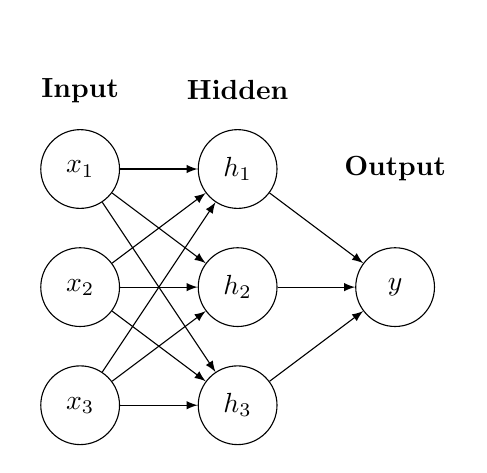
\begin{tikzpicture}[node distance=1cm and 1.5cm,
        every node/.style={circle, draw, minimum size=1cm},
        every path/.style={->, >=latex}]
        
      % Input layer
      \node (I1) at (0,3) {$x_1$};
      \node (I2) at (0,1.5) {$x_2$};
      \node (I3) at (0,0) {$x_3$};
  
      % Hidden layer
      \node (H1) at (2,3) {$h_1$};
      \node (H2) at (2,1.5) {$h_2$};
      \node (H3) at (2,0) {$h_3$};
  
      % Output layer
      \node (O1) at (4,1.5) {$y$};
  
      % Connections Input -> Hidden
      \foreach \i in {1,2,3}
        \foreach \h in {1,2,3}
          \draw (I\i) -- (H\h);
  
      % Connections Hidden -> Output
      \foreach \h in {1,2,3}
        \draw (H\h) -- (O1);
  
      % Layer labels
      \node[draw=none] at (0,4) {\textbf{Input}};
      \node[draw=none] at (2,4) {\textbf{Hidden}};
      \node[draw=none] at (4,3) {\textbf{Output}};
    \end{tikzpicture}
    \caption{A simple MLP with one hidden layer.}
    \label{fig:2layer_mlp}
  \end{wrapfigure}

%TODO: consisting of multiple layers of hidden units and nonlinear activation functions
A classical DL model is the \ac{MLP}, first proposed by Rosenblatt~\cite{rosenblatt1958perceptron}, with the general goal of approximating a function $f^*$. In the case of classification we could define a function $y = f^*(\mathbf{x})$ that maps an input vector $\mathbf{x}$ to a label $y$. The MLP then defines the mapping $y = f(\mathbf{x};\boldsymbol{\theta})$ and learns the value of the parameters $\boldsymbol{\theta}$ that best approximate the function. At the start of the training these parameters are initialized randomly or by a smart initialization strategy, like the Glorot/Xavier~\cite{glorot2010understanding} initialization. \bigskip

These models are also referred to as feedforward neural networks, as they process information from $\mathbf{x}$, through the intermediate computations that define $f$, to the output $y$ without feedback connections that would feed outputs back to itself. The name network is derived from their representation as a composition of multiple different functions, that are described by a directed acyclic graph. An example network is $f(\mathbf{x}) = f^{(2)}(f^{(1)}(\mathbf{x}))$, which processes an input vector $\mathbf{x}$ through a hidden layer $f^{(1)}$, and an output layer $f^{(2)}$ (see Figure \ref{fig:2layer_mlp}).  The length of this chain of functions defines the depth of a model, coining the term "deep learning". 

The approximation is achieved by training our network with training data, that consists of approximated examples of $f^*(\mathbf{x})$ at different points in the training, and labels $y\approx f^*(\mathbf{x})$. These training examples dictate the output layer to generate a value close to $y$ for each input $\mathbf{x}$, or to produce a higher-level representation that can be used for subsequent tasks. The learning algorithm then learns to utilize the other hidden layers, without specified behaviors, to achieve the best approximation. It is to note that the hidden layers are vector-valued with each vector element, referred to as unit, loosely taking the role of a neuron in neuroscience. This comparison is a common analogy to convey the idea of information processing. Models are therefore also referred to as neural networks. \bigskip

%We use non-linear activation functions in layers to describe features and keep the model from learning a strictly linear transformation of its inputs. Result for a layer is vector of hidden units $h=g(W^Tx+b)$, where $W$ contains the weights of a linear transformation and b the biases. x is the input vector. $g$ is the activation function that is usually applied element-wise, such as ReLU or Sigmoid.

Following \cite{Goodfellow-et-al-2016}, an input or intermediate layer for our model could be defined as
\begin{equation}
    f^{(i)}(\mathbf{x}; \mathbf{W},\mathbf{c})=\mathbf{W}^\top\mathbf{x}+\mathbf{c},
\end{equation}
where $\mathbf{W} \in \mathbb{R}^{m\times d}$ denotes a weight matrix for $m$ units with $d$ features and $\mathbf{c}\in \mathbb{R}^m$ is a vector of bias terms.
To keep the model from strictly learning a linear function of its inputs we can calculate the vector of hidden units $\mathbf{h}$ by applying an activation function $g$ to the output of the linear layer:
\begin{align}
    \mathbf{h} = g(f^{(i)}(\mathbf{x}; \mathbf{W},\mathbf{c})).
\end{align}
The activation function $g$ is typically applied element-wise to describe the features of a hidden layer:
\begin{equation}
    h_i = g(\mathbf{x}^\top\mathbf{W}_{:,i}+c_i).
\end{equation}
The hidden units $\mathbf{h}$ can then serve as input to the next hidden layer or directly to the output layer.

An example for a linear output layer that calculates a scalar for an input vector $\mathbf{h}$ is
\begin{equation}
    f^{(i+1)}(\mathbf{h}; \mathbf{w},b)=\mathbf{h}^\top\mathbf{w}+b,
\end{equation}
with weight vector $\mathbf{w} \in \mathbb{R}^d$ and bias $b \in \mathbb{R}$ as parameters. This would define our model consisting of the two defined layers as $f(x;\boldsymbol{\theta})$ with parameters $\boldsymbol{\theta} = (\mathbf{W}, \mathbf{c}, \mathbf{w}, b)$. The learning algorithm would thus adapt the parameters $\boldsymbol{\theta}$ to approximate the target function as close as possible.

The activation function typically maps its input to a real number within a specific range, often between $0$ and $1$, conceptually imitating the activation of a biological neuron. We try to use activation functions that are continuous differentiable and easily calculated, to minimize computational complexity \cite{Liu2020}. Examples are the Sigmoid function

%GNN BOOK: \\
%initiated with random weights or values, updated in each neuron with backpropagation. Learned knowledge stored in connections digitally. \\
%Each neuron therefore takes inputs $x_1, ..., x_n$ with corresponding weights $w_1, ..., w_n$ and an offset $b$. A layer can then be described as a linear function $y=\sum_{i=1}^{n} w_i x_i +b$ that is optionally passed through a non-linear activation function $f$ that generates the output of the current layer $z = f(y)$. The activation function usually serves the purpose of mapping to a real number between $0$ and $1$, imitating the activation of a neuron. We try to use activation functions that are continuous differentiable and easily calculated, to minimize computational complexity. Examples are the Sigmoid function 
\begin{equation}
    \sigma (x)= \frac{1}{1+e^{-x}},
\end{equation}
where $e$ denotes the exponential function, and the Rectified Linear Unit (ReLU):
\begin{equation}
    ReLU(x)=\begin{cases}
        0 & x \leq 0, \\
        1 & x > 0.
    \end{cases}
\end{equation}
\bigskip

\textbf{Backpropagation}\par
The backpropagation algorithm \cite{rumelhart1986learning} is commonly used during neural network training. It optimizes the network parameters by leveraging gradient descent. It first calculates the values for each unit in the network given the input and a set of parameters in a forward order. Then the error for each variable to be optimized is calculated, and the parameters are updated according to their corresponding partial derivative backwards. These two steps will repeat until reaching the optimization target \cite{Goodfellow-et-al-2016}.

\subsection{Regularization}
A central problem of not only DL but ML in general is the creation of an algorithm that generalizes well, therefore performing not only on training data, but also on unseen test inputs \cite{Goodfellow-et-al-2016}. There exists many strategies that aim to reduce the test error, sometimes at the expense of an increase in training error. These strategies are known as regularization. We introduce a selection of these strategies that are relevant in the course of this work, following Goodfellow et al.~\cite{Goodfellow-et-al-2016}.\bigskip

\textbf{Parameter Norm Penalties}\par
Many regularization approaches in DL restrict the capacity of a model by adding a parameter norm penalty $\Omega(\boldsymbol{\theta})$ to the objective function. Let $J$ be the objective function of our learning algorithm, with training input $\mathbf{X} \in \mathbb{R}^{I\times d}$ and target values $\mathbf{y} \in \mathbb{R}^I$, for $I$ training instances with $n$ features. The regularized objective function is then defined as
\begin{equation}
    \tilde{J}(\boldsymbol{\theta}; \mathbf{X}, \mathbf{y}) = J(\boldsymbol{\theta}; \mathbf{X}, \mathbf{y}) + \alpha\Omega(\boldsymbol{\theta}),
\end{equation}
where $\alpha \in [0,\infty)$ is a hyperparameter used to weigh the relative contribution of the norm penalty term $\Omega(\boldsymbol{\theta})$. $\alpha=0$ results in no regularization, while larger values increase the regularization effect. During training the algorithm will not only minimize the objective function $J$, but also the regularization measure of the parameters $\boldsymbol{\theta}$, or a subset of these. We usually only regularize the weights $\mathbf{w}$ with $\Omega$, since these specify the interaction of two variables, rather than the bias $b$ that only controls a singular variable \cite{Goodfellow-et-al-2016}.

Inherently, different parameter norms $\Omega$ can result in different preferred solutions. One common example is the $L^2$ regularization, known as weight decay. It drives the weights closer to the origin by adding the term
\begin{equation}
    \Omega(\boldsymbol{\theta}) = \frac{1}{2}||\mathbf{w}||_2^2 = \frac{1}{2}\mathbf{w}^\top \mathbf{w},
\end{equation}
with $||\mathbf{x}||_p = (\sum_i |x_i|^p)^\frac{1}{p}$ denoting the $L^p$ norm or size of a vector $\mathbf{x}$. Specifically, the $L^2$ norm denotes the Euclidean distance from the origin to the point $\mathbf{x}$, and the size of a vector $\mathbf{x}$ if squared: $||\mathbf{w}||_2^2 = \mathbf{x}^\top \mathbf{x}$. \bigskip

Another option is the $L^1$ regularization, defined as
\begin{equation}
    \Omega(\boldsymbol{\theta}) = ||\mathbf{x}||_1 = \sum_i |\mathbf{x}_i|,
\end{equation}

that provides a more sparse solution in comparison, meaning that some parameters have an optimal value of zero. \bigskip

\textbf{Early stopping}\par
When training a deep model, a commonly observable problem is the training error steadily decreasing over time, but the validation set error rising after some time, indicating that the model is overfitting to the train data \cite{Goodfellow-et-al-2016}. To obtain a better model we may then return to a parameter setting at an earlier point in the training, where the validation set error was at its lowest. In practice, we store a copy of the model parameters at any point in training where the validation error decreases. Thus, when the training is concluded we return the stored set of parameters, rather than the latest one. Additionally, we may stop our algorithm early if the validation error does not decrease over a set period of iterations.\bigskip

\textbf{Dropout}\par
Dropout~\cite{hinton2012improving} is a regularization technique used to prevent a neural network from "overfitting" to the training data, which occurs due to feature detectors of models being highly tuned to the training data, but not to the unseen test data. This is done by randomly omitting each hidden unit from the network with a common probability $p$ for each presentation of each training instance, to avoid hidden units relying on the presence of other hidden units. Usually, to reduce the error on a test set, an average of the predictions of multiple networks is consulted, which requires training many separate networks. Random dropout provides a computationally cheap alternative to this approach. Effectively, at each presentation of each training instance a different network is used, but the present hidden units share the same weights across all these networks.

At test time, the "mean network" is used, that contains all hidden units with their outgoing weights scaled by the factor $\frac{1}{1-p}$, to account for more hidden units being present during this stage. \bigskip

\textbf{Batch Normalization}\par
While not strictly a regularization technique, batch normalization~\cite{ioffe2015batch} often serves a similar purpose in practice by improving generalization.
In deep models composed of several layers the gradient tells us how to update each parameter assuming that the other layers do not change. Since in practice all layers are updated simultaneously, this may lead to unexpected results. Batch normalization is an optimization technique that can be applied to any input or hidden layer to reduce the aforementioned problem. We follow the definition by Goodfellow et al.~\cite{Goodfellow-et-al-2016}.

Let $\mathcal{B}$ be a mini-batch of activations of the layer to normalize, in the form of a design matrix with rows of activations. To normalize $\mathcal{B}$, it is replaced by
\begin{equation}
    \mathcal{B}' = \frac{\mathcal{B} - \boldsymbol{\mu}}{\boldsymbol{\sigma}},
\end{equation}
where $\boldsymbol{\mu}$ is a vector containing the mean of each unit and $\boldsymbol{\sigma}$ is a vector containing the standard deviation of each unit. Each activation is normalized individually with the $\boldsymbol{\mu}$ and $\boldsymbol{\sigma}$ corresponding to its row. The network processes $\mathcal{B}'$ as functionally equivalent to $\mathcal{B}$. During training,
\begin{equation}
    \boldsymbol{\mu} = \frac{1}{m}\sum_i \mathcal{B}_i
\end{equation}
and
\begin{equation}
    \boldsymbol{\sigma} = \sqrt{\delta + \frac{1}{m} \sum_i (\mathcal{B}_i - \boldsymbol{\mu})^2},
\end{equation}

where $\delta$ is a small positive value introduced to avoid $\sqrt{z}$ at $z = 0$ and $m$ is the number of elements in the batch. It is important to note that backpropagation is performed through all three operations, to prevent the gradient from proposing an operation that solely increases the mean and standard deviation of the output of a layer. Batch normalization therefore reparameterizes the model to include some units that are standardized by definition.

When testing the model, we replace $\boldsymbol{\mu}$ and $\boldsymbol{\sigma}$ with running averages that were collected during training, to enable the evaluation of individual examples outside mini-batches.

\subsection{Monte Carlo Sampling}
In order to best approximate a randomized algorithm we can make use of Monte Carlo methods as described in \cite{Goodfellow-et-al-2016}. A common practice in ML is to draw samples from a probability distribution and using these to form a Monte Carlo estimate of some quantity. This can be used to train a model that can then sample from a probability distribution itself. \bigskip
More specifically, the idea of Monte Carlo sampling is to view a sum of function evaluations, such as those of a loss function, as if it was an expectation under some probability distribution. This estimate is approximated with a corresponding average. Let $X$ be a discrete random variable with alphabet $\mathcal{X}$ and probability mass function $p(x)=Pr\{X=x\}$ for $x\in \mathcal{X}$. The sum to estimate is defined as
\begin{equation}
    s = \sum_{x\in \mathcal{X}} p(x)f(x)=\mathbb{E}_p[f(X)],
\end{equation}
where $\mathbb{E}$ denotes the expectation. Then $s$ can be approximated by drawing $n$ samples from $p$ and constructing the empirical average 
\begin{equation}
    \hat{s}_n=\frac{1}{n}\sum_{i=1}^n f(x^{(i)}).
\end{equation}


\section{Graph Theory}
\label{sec:graph_theory}
The following definitions loosely follow Liu and Zhou~\cite{Liu2020}. A graph is a data structure consisting of a set of nodes that are connected via edges, modeling objects and their relationships. It can be represented as $G=(V,E)$ with $V=\{v_1,v_2...v_n\}$ being the set of $n$ nodes, and $E \subseteq V \times V$ being the set of edges. We adopt the conventions from Diestel~\cite{Diestel2017} to refer to the node and edge set of any graph $G$ with $V(G)$ and $E(G)$ respectively, regardless of the actual names of the sets. Moreover, we refer to $G$ with node set $V$ as "$G$ on $V$". \bigskip

An edge $e=(u,v)$, connects nodes $u$ and $v$, making them neighbors that are both incident to $e$. The neighborhood $\mathcal{N}(u)$ of node $u$ in $V(G)$ is defined as 
\begin{equation*}
    \mathcal{N}(u) = \{v \in V(G) \mid (v,u) \in E(G)\}.
\end{equation*} 
We denote the set of edges that are incident to $u$ as 
\begin{equation*}
    E(u) = \{(v,u) \in E(G) \mid v \in \mathcal{N}(u)\}.
\end{equation*}
Additionally, we define the $k$-hop neighborhood of node $u$ in $V(G)$ as 
\begin{equation*}
    \mathcal{N}_k(u) = \{v \in V(G) \mid \text{dist}_G(v,u) \leq k\},
\end{equation*}
where $\text{dist}_G(v,u)$ denotes the distance of nodes $v, u$ in $G$, defined as the length of the shortest path between the two nodes. Edges are either directed or undirected and lead to directed or undirected graphs if exclusively present. \bigskip

The degree of a node $v \in V(G)$ is the number of edges connected to $v$ and denoted by $d(v) = |\{(u,v) \in E(G) \mid u \in V(G)\}|$. $G$ can be described by an adjacency matrix $\mathbf{A} \in \mathbb{R}^{n \times n}$, where
\begin{equation*}
    \mathbf{A}_{ij}=\begin{cases}
        1 & \text{if } \{v_i,v_j\}\in E \text{ and } i \neq j, \\
        0 & \text{otherwise.}
    \end{cases}
\end{equation*}
If $G$ is an undirected Graph the adjacency matrix will be symmetrical, as seen in Figure \ref{fig:graph-example}.
%Alternatively an undirected graph $ G=(V, E)$ with $n$ nodes and $m$ edges can be represented as an incidence matrix $M \in \mathbb{R}^{n \times m}$, where
%\begin{equation*}
%    M_{ij}=\begin{cases}
%        1 & \text{if } \exists k \text{ s.t. } e_j = \{v_j, v_k\}, \\
%        0 & \text{otherwise.}
%    \end{cases}
%\end{equation*}
The diagonal degree matrix $D\in \mathbb{R}^{n\times n}$ of $G$ is defined as:
\begin{equation*}
    D_{ii} = d(v_i).
\end{equation*}

$G$ is called a subgraph of another graph $G'=(V',E')$, denoted as $G' \subseteq G$, if 
\[
    V(G) \subseteq V(G') \text{ and } E(G) \subseteq E(G').
\]
The number of nodes $|V|$ in a graph is called its order and the number of edges $|E|$ is its size (see Diestel~\cite{Diestel2017}). \bigskip

We follow the definition of bipartite graphs given by Asratian et al.~\cite{asratian1998}: A graph $G$ is bipartite if the set of nodes $V$ can be partitioned into two disjoint sets $V_1$ and $V_2$ such that
\begin{align*}
    &V = V_1 \cup V_2,\quad V_1 \cap V_2 = \emptyset, \quad \text{and} \\
    &\forall (i,j) \in E(G):\ (i \in V_1 \land j \in V_2) \lor (i \in V_2 \land j \in V_1).
\end{align*}
This formalizes that no two nodes from the same set are adjacent. The sets $V_1$ and $V_2$ are called color classes and $(V_1, V_2)$ is a bipartition of $G$. This means that if a graph is bipartite all nodes in $V$ can be colored by at most two colors so that no two adjacent nodes share the same color. This is visualized in Figure \ref{fig:bipartite-colored}. \bigskip
\begin{figure}[h]
    \centering
    \begin{minipage}{0.5\textwidth}
        \centering
        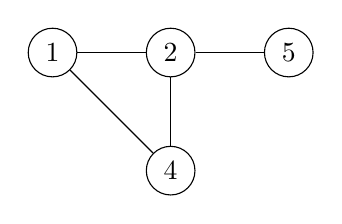
\begin{tikzpicture}[node distance=1.5cm, every node/.style={draw, circle}]
            % Define Nodes
            \node (1) {1};
            \node (2) [right of=1] {2};
            \node (4) [below of=2] {4};
            \node (5) [right of=2] {5};
            
            % Draw Edges
            \draw (1) -- (2);
            \draw (2) -- (4);
            \draw (1) -- (4);
            \draw (2) -- (5);
        \end{tikzpicture}
    \end{minipage}%
    \begin{minipage}{0.45\textwidth}
        \vspace*{0.1cm} % Adjust this value to fine-tune vertical alignment
        \[
        \mathbf{A} = \begin{bmatrix}
            0 & 1 & 1 & 0 \\
            1 & 0 & 1 & 1 \\
            1 & 1 & 0 & 0 \\
            0 & 1 & 0 & 0 \\
        \end{bmatrix}
        \]
    \end{minipage}
    \caption[Example of an undirected graph]{A simple undirected graph $G$ on $V$, with $V=\{1,2,4,5\}$ (left), and its adjacency matrix $\mathbf{A}$ (right).}
    \label{fig:graph-example}
\end{figure}

\begin{figure}[h]
    \centering
    \begin{tikzpicture}[
        every node/.style={circle, draw, minimum size=1cm},
        on grid,
        node distance=2cm
    ]
        % Define nodes in two color classes
        \node[fill=blue!20] (u1) at (0,0) {1};
        \node[fill=blue!20] (u2) at (2,0) {2};
        \node[fill=blue!20] (u3) at (4,0) {3};

        \node[fill=red!20] (v1) at (1,-2) {a};
        \node[fill=red!20] (v2) at (3,-2) {b};

        % Edges between classes
        \draw (u1) -- (v1);
        \draw (u1) -- (v2);
        \draw (u2) -- (v1);
        \draw (u3) -- (v2);
    \end{tikzpicture}
    \caption[Example of a bipartite graph]{A bipartite graph with color classes $V_1 = \{1,2,3\}$ (blue) and $V_2=\{a,b\}$ (red).}
    \label{fig:bipartite-colored}
\end{figure}

\textbf{Random Graphs}\par
\label{sec:random-graphs}
%Gilbert\cite{} describes the process of generating a random graph of order $N$ by assigning a common probability to exist in the graph to each potential edge between two nodes. Note that these random selections are made independently of each other, effectively drawing from a Bernoulli distribution. \\
Gilbert~\cite{gilbert1959random} describes the process of generating a random graph of order $n$ by assigning a common probability of existence to each potential edge between any two nodes. For each of these potential edges an experiment is performed independently to determine whether it shall be included in the resulting graph. Note that this process can be modeled using a Bernoulli distribution.
%The actual edges in the graph are then selected by performing random experiments, made independently of each other, and can therefore be described by a Bernoulli distribution.
%Note that these random selections are made independently of each other and effectively drawn from a Bernoulli distribution.

%Version 1 (probability space for PGE not needed, definition for one random graph suffices?): \\
A random graph is further described by Diestel~\cite{Diestel2017} as follows. Let $V = \{0,...,n-1\}$ be a fixed set of $n$ elements. Say we want to define the set $\mathcal{G}$ of all graphs on $V$ as a probability space, which allows us to ask whether a Graph $G \in \mathcal{G}$ has a certain property. To generate our random graph we then decide from some random experiment whether $e$ shall be an edge of $G$ for each potential $e \in V \times V$. The probability of success - accepting $e$ as edge in $G$ - is defined as $p \in [0,1]$ for each experiment. This leads to the probability of $G$ being a particular graph $G_0$ on $V$ with e.g. $m$ edges being equal to $p^m q^{\binom{n}{2}-m}$ with $q:=1-p$.
\bigskip

%Version 2: \\
%A random graph is further described by Diestel\cite{Diestel2017}[p.323] as follows. Let $V = \{0,...,n-1\}$ be a fixed set of $n$ elements. To generate our random graph we then decide from some random experiment whether $e$ shall be an edge of $G$ for each potential $e \in V \times V$. The probability of success - accepting $e$ as edge in $G$ - is defined as $p \in [0,1]$ for each experiment. This leads to the probability of $G$ being a particular graph $G_0$ on $V$ with e.g. $m$ edges being equal to $p^m q^{\binom{n}{2}-m}$ with $q:=1-p$. It follows our desired probability space $\mathcal{G}=(n,p)$ as the product space
%\begin{equation}
%    \Omega := \prod_{e \in [V]^2} \Omega_e
%\end{equation}
%with $\Omega_e := \{0_e,1_e\}$, $\mathbb{P}_e(\{1_e\}) := p$ and $\mathbb{P}_e(\{0_e\}) := q$.
%TODO: This is probably unnecessary for PGE.
%\begin{equation}
%    E(G) = \{e | \omega(e) = 1_e\}
%\end{equation}
%E(G) = Edges of G. G is called a random graph on V with edge probability $p$. \bigskip

\section{Information Theory}
\label{sec:information_theory}
To fully understand the learning objective of PGExplainer it is necessary to define the concepts of entropy and mutual information. We follow the definitions by Cover and Thomas~\cite{Cover2005} if not stated otherwise.

\subsection{Entropy}
%TODO: REVISE THIS. Probably best to define with general expactation, for continous and discrete, according to Goodfellow. Derive conditional entropy for general case. Only apply discrete case where needed? (cross entropy in PGE) \bigskip

Entropy is used to describe the uncertainty of a random variable. It quantifies the average amount of information produced by the outcomes of said variable. This is commonly illustrated as the average number of bits needed to encode its possible values if optimal code is used \cite{Goodfellow-et-al-2016}.
The entropy $H(X)$, also written as $H(p)$, is defined as
\begin{equation}
    H(X) = -\sum_{x \in \mathcal{X}} p(x) \log p(x).
\end{equation}
%TODO: WE USE NATURAL LOGARITHM IN CODE!
The log is to the base $e$ and entropy is measured in natural units of information (nats) in our case. We will use the convention from Cover and Thomas~\cite{Cover2005} that $0 \log 0 = 0$, as terms of zero probability do not change the entropy. %A simple example is tossing two coins: There are four possible outcomes $\mathcal{X}=\{00,10,01,11\}$, 0 for heads and 1 for tails, each with a probability $p=0,25$. The resulting entropy $H(X)=2$ represents that two bits of information can be stored this way. \bigskip
\\
%TODO: DIFFER MORE CLEARLY FROM CROSS? \\
%Analogously we define the joint entropy $H(X,Y)$ of a pair of discrete random variables $(X,Y)$ with a joint distribution $p(x,y)$ as follows:
%\begin{equation}
%    H(X,Y)=-\sum_{x \in \mathcal{X}} \sum_{y \in \mathcal{Y}} p(x,y) \log p(x,y).
%\end{equation}
The conditional entropy of $Y$ given $X$ is defined as the expected value of the entropies of the conditional distributions, averaged over the conditioning random variable. Let $(X,Y) \sim p(x,y)$ for a pair of discrete random variables $(X,Y)$ with joint distribution $p(x,y)$. The conditional entropy is then defined as
\begin{align}
    H(Y|X)&= -\sum_{x \in \mathcal{X}} p(x) H(Y|X=x) \nonumber \\
    &= - \sum_{x \in \mathcal{X}} \sum_{y \in \mathcal{Y}}p(x,y) \log p(y|x) \nonumber \\
    &= -\mathbb{E} \log p(Y|X). \label{eq:cond_ent}
\end{align}

\subsection{Relative Entropy and Cross-Entropy}
%Elements of Information Theory: equation 2.26 describes KL distance/relative entropy \bigskip
The relative entropy between two distributions is a measure of "distance" between the two. It measures the inefficiency of assuming a distribution to be $q$ when the true distribution is $p$. Note that it is not a true measure of distance as it is not symmetrical. The relative entropy takes a value of $0$ only if $p = q$.
We define the KL divergence or relative entropy between two probability mass functions $p(x), q(x)$ as
\begin{equation}
    D_{KL}(p||q) = \sum_{x \in \mathcal{X}} p(x)\log \frac{p(x)}{q(x)}.
\end{equation}
We adopt the convention from Cover and Thomas~\cite{Cover2005} that $0 \log \frac{0}{0} = 0$, $0 \log \frac{0}{q} = 0$ and $p \log \frac{p}{0} = \infty$.
Suppose we know the true distribution $p$ of our random variable. We could then construct a code with an average description length of $H(p)$. If we used the code for the distribution $q$ instead, we would need $H(p) + D_{KL}(p||q)$ nats to describe the random variable on average. This is also referred to as the cross-entropy (see Goodfellow et al.~\cite{Goodfellow-et-al-2016}):
\begin{equation}
    H(p,q) =  H(p) + D_{KL}(p||q)
\end{equation}


%The following definitions loosely follow Goodfellow et al.\cite{Goodfellow-et-al-2016}[p.74].
%The relative entropy is a measure of the distance between two distributions.
%"measure how different these two distributions are" \cite{Goodfellow-et-al-2016}
%"In the case of discrete variables, it is the extra amount of information needed to send a message containing symbols drawn from probability distribution P, when we use a code that was designed to minimize the length of messages drawn from probability distribution Q."
%"The KL divergence is 0 if and only if P and Q are the same distribution in the case of discrete variables"
%non symmetrical.
%"When computing many of these quantities, it is common to encounter expressions of the form 0 log 0. By convention, in the context of information theory, we treat these expressions as limx→0 x log x = 0. \\
%We define the KL divergence or relative entropy between two probability distributions $P, Q$ as
%\begin{equation}
%    D_{KL}(P||Q) = \sum_{x \in \mathcal{X}} P(x)\log \frac{P(x)}{Q(x)}
%\end{equation}

%The cross entropy is closely related to KL distance and therefore defined as
%\begin{align}
%    H(P,Q) &= -\mathbb{E}_{x\sim P}\log Q(x) \\
%    &= H(P) + D_{KL}(P||Q)
%\end{align}

Since this is later applied in the PGExplainer (see Equation \ref{eq:monte_carlo}), we derive for the discrete case with mass probability functions $p, q$ defined on the same support $\mathcal{X}$:
\begin{align}
    H(p,q) = H(p) + D_{KL}(p||q) 
    &= -\sum_{x \in \mathcal{X}} p(x) \log p(x) + \sum_{x \in \mathcal{X}} p(x)\log \frac{p(x)}{q(x)} \nonumber \\
    &= -\sum_{x \in \mathcal{X}} p(x) \log p(x) + \sum_{x \in \mathcal{X}} p(x) \log p(x) -\sum_{x \in \mathcal{X}} p(x) \log q(x) \nonumber \\
    &= -\sum_{x \in \mathcal{X}} p(x) \log q(x) \label{eq:cross_entropy}
\end{align}

\subsection{Mutual Information}
%(see Cover et al.\cite{Cover2005}[p.19])
A closely related concept is mutual information. It measures the amount of information that one random variable contains about another or the reduction in uncertainty of said variable due to knowing the other. A high mutual information therefore implies that the information of one variable can be gathered from the other.

Let $X$ and $Y$ be two random variables with the joint probability mass function $p(x,y)$ and marginal probability mass functions $p(x)$ and $p(y)$. Mutual information $MI(X;Y)$ is the relative entropy between the joint distribution and the product distribution $p(x)p(y)$: 
\begin{align}
    MI(X;Y)&=\sum_{x \in \mathcal{X}}\sum_{y \in \mathcal{Y}} p(x,y)\log \frac{p(x,y)}{p(x)p(y)} \nonumber \\
    &= H(X) - H(X|Y) \label{eq:mutual_information}
\end{align}

\section{Graph Neural Networks}
\label{sec:gnns}

\acp{GNN} \cite{4700287} are a DL-based approach for modeling graph data. Due to their unique non-Euclidean property they find usage in many areas, with common tasks including node classification \cite{gao2019graph}, graph classification \cite{xu2018powerful} and link prediction \cite{zhang2018link}. Their high interpretability and strong performance have led to GNNs becoming a commonly employed method in graph analysis. Modern GNNs combine the key features of convolutional neural networks \cite{726791}, such as local connection, shared weights, and multi-layer usage, with the concept of graph embeddings \cite{cai2018comprehensive} to leverage the power of feature extraction and representation as low-dimensional vectors for graphs (see Liu and Zhou~\cite{Liu2020}).\bigskip

TODO: CONCRETELY DEFINE NODE AND GRAPH TASKS! VISUALIZE?
Graphs are a common way of representing data in many different fields, including ML. ML applications on graphs can mostly be divided into graph-focused tasks and node-focused tasks. For graph-focused applications our model does not consider specific singular nodes, but rather implements, for example, a classifier on representations of complete graphs. In node-focused applications however the model is dependent on specific nodes, leading to classification tasks that rely on the properties of each node.

The study of GNNs was first introduced in \cite{gori2005new} and refined in \cite{4700287}. Thus, we describe the supervised GNN model by Scarselli et al.~\cite{4700287} that aims to preserve the important, structural information of graphs by encoding their topological relationships among nodes. \bigskip

A node is naturally defined by its features as well as its related nodes in a graph. The goal of a GNN is to learn state embeddings $\mathbf{h}_v \in \mathbb{R}^d$ for each node $v$, that map the neighborhood of a node into a representation. These embeddings are used to obtain outputs $\mathbf{o}_v$, that, e.g., may contain the distribution of a predicted node label. The GNN model proposed by Scarselli et al.~\cite{4700287} uses undirected homogeneous graphs with $\mathbf{x}_v$ describing the $d$-dimensional features of each node and $x_e$ the optional features of each edge. The model updates the node states according to the input neighborhood with a local transition function $f$ that is shared by all nodes. Additionally, the local output function $g$ is used to produce the output of each node. $\mathbf{h}_v$ and $\mathbf{o}_v$ are therefore defined as
\begin{equation}
    \mathbf{h}_v = f(\mathbf{x}_v, \mathbf{x}_{E(v)}, \mathbf{h}_{\mathcal{N}(v)}, \mathbf{x}_{\mathcal{N}(v)}),
    \label{eq:gnn_state_local}
\end{equation}
\begin{equation}
    \mathbf{o}_v = g(\mathbf{h}_v, \mathbf{x}_v),
\end{equation}
with $\mathbf{x}$ denoting input features and $\mathbf{h}$ the hidden state. $\mathbf{x}_v, \mathbf{x}_{E(v)}, \mathbf{h}_{\mathcal{N}(v)}, \mathbf{x}_{\mathcal{N}(v)}$ denote the features of the node $v$ and of its incident edges, as well as the states and features of its neighboring nodes, respectively. We define $\mathbf{H}, \mathbf{O}, \mathbf{X} \text{ and  }\mathbf{X}_N$ as the matrices that are constructed by stacking all states, outputs, features, and node features, respectively. This allows us to define with the global transition function $F$ and the global output function $G$, which are stacked versions of their local equivalent for all nodes in a graph: 
\begin{equation}
    \mathbf{H} = F(\mathbf{H}, \mathbf{X}),
    \label{eq:gnn_state_global}
\end{equation}
\begin{equation}
    \mathbf{O} = G(\mathbf{H},\mathbf{X}_N).
\end{equation}
Note that $F$ is assumed to be a contraction map and the value of $\mathbf{H}$ is the fixed point of equation \eqref{eq:gnn_state_global}. To compute the state the iterative scheme
\begin{equation}
    \label{eq:GNN_iterations}
    \mathbf{H}^{t+1} = F(\mathbf{H}^{t}, \mathbf{X})
\end{equation}
is used with $\mathbf{H}^{t}$ denoting iteration t of $\mathbf{H}$. The computations of $f$ and $g$ can be understood as the feedforward neural network. \\
To learn the parameters of this GNN, with target information $t_v$ for a specific node $v$, the loss is defined as
\begin{equation}
    loss = \sum_{i=1}^p (t_i-\mathbf{o},)
\end{equation}
where $p$ are the supervised nodes. A gradient-descent strategy is utilized in the learning algorithm, which consist of the following three steps: the states $\mathbf{h}_v^{t}$ are updated iteratively using equation \eqref{eq:gnn_state_local} until time step $T$. We then obtain an approximate fixed point solution of equation \eqref{eq:gnn_state_global}: $\mathbf{H}(T)\approx\mathbf{H}$. For the next step the gradients of the weights $W$ are calculated from the loss. Finally, the weights $W$ are updated according to the computed gradient. This allows us to train a model for specific supervised or semi-supervised tasks, referred to as downstream task, and get hidden states of nodes in a graph \cite{Liu2020}. \bigskip

Though the architecture proposed by Scarselli et al.~\cite{4700287} proved to be powerful for modeling structural data, this initial approach suffers from a few limitations. Most notably, it uses the same parameters in the iteration, while nowadays it is common practice to use different parameters in different layers \cite{Liu2020}. 

Stacking $k$ GNN layers allows each node to aggregate information from nodes within its $k$-hop neighborhood, represented in Figure \ref{fig:k-hop}, seeking an increase in performance. It is important to note that this approach may also increase the noisy information spread by the exponentially increasing neighborhood nodes \cite{Liu2020}.

Another drawback is the computational inefficiency, as hidden states have to be updated $T$ times until reaching the fixed point. A relaxation of the fixed point assumption enables multi-layer GNNs to provide stable representations of the node and its neighborhood \cite{li2015gated}. Additionally, this architecture is unable to model informative edge features, which limits its capacity to learn meaningful hidden representations for edges.

\tikzstyle{texts} = [text centered, font=\small, draw=none]
\begin{figure}
    \centering
    \begin{tikzpicture}[scale=1.2, every node/.style={circle, draw, minimum size=8mm, inner sep=1pt}]
        % Central node
        \node[fill=blue!30] (u) at (0,0) {$u$};
    
        % 1-hop neighbors (green)
        \foreach \i/\name in {0/v1, 90/v2, 180/v3, 270/v4} {
            \node[fill=green!30] (\name) at (\i:2) {$\name$};
            \draw (u) -- (\name);
        }
    
        % 2-hop neighbors (yellow)
        \foreach \i/\name in {20/w1, 110/w3, 160/w4, 200/w5, 250/w6, 290/w7, 340/w8} {
            \node[fill=yellow!30] (\name) at (\i:3.5) {$\name$};
        }
    
        % Connections from 1-hop to 2-hop
        \foreach \parent/\child in {v1/w1, v2/w3, v2/w4, v3/w5, v3/w6, v4/w7, v4/w8} {
            \draw (\parent) -- (\child);
        }

        % Highlight 2-hop neighborhood
        \begin{scope}[on background layer]
            \fill[yellow!10] (0,0) circle (4);
            \fill[green!10] (0,0) circle (2.4);
        \end{scope}

        % Labels directly on the rings
        \node[texts, font=\small] at (45:2.4) {1-hop neighborhood};
        \node[texts, font=\small] at (45:4) {2-hop neighborhood};
        
    \end{tikzpicture}
    \caption[$k$-hop neighborhood visualization]{Visualization of the $k$-hop neighborhood of $u$.}
    \label{fig:k-hop}
\end{figure}

Therefore, we briefly present two subsequent models that are used in the course of this work, as well as a more general framework relevant in the context of NeuroSAT. \bigskip

\textbf{Graph Convolutional Network} \par
The \ac{GCN} aims to generalize the convolution operation of \acp{CNN} to the graph domain. An example is the model proposed by Kipf and Welling~\cite{kipf2016semi} that introduces a simple, layer-wise propagation rule for multi-layer GCNs as
\begin{equation}
    \label{eq:GCN}
    \mathbf{H}^{(l+1)} = \sigma(\tilde{\mathbf{D}}^{-\frac{1}{2}}\tilde{\mathbf{A}}\tilde{\mathbf{D}}^{-\frac{1}{2}}\mathbf{H}^{(l)}\mathbf{W}^{(l)}),
\end{equation}
where $\tilde{\mathbf{A}} = \mathbf{A} + \mathbf{I}_N$ is the adjacency matrix of the undirected input graph $G$ with added self-connections. $\mathbf{I}_N$ is the identity matrix, $\tilde{\mathbf{D}}$ is the degree matrix and $\mathbf{W}^{(l)}$ is a layer-specific trainable weight matrix. $\sigma(\cdot)$ denotes an activation function, such as ReLU. $\mathbf{H}^{(l)} \in \mathbb{R}^{n\times d}$ denotes the matrix of node activations in the $l$-th layer, where $\mathbf{H}^{(0)} = X$. 

Note that this definition differs from the iterative formulation in Equation \ref{eq:GNN_iterations}, in the sense that each layer applies a different function $F^{(l)}$, rather than a shared function $F$. $\tilde{\mathbf{D}}^{-\frac{1}{2}}\tilde{\mathbf{A}}\tilde{\mathbf{D}}^{-\frac{1}{2}}$ describes a normalization of the adjacency matrix, referred to as renormalization trick. This architecture aims to alleviate the problem of overfitting on local neighborhood structures for graphs with very wide node degree distributions \cite{kipf2016semi}. \bigskip

%TODO: generalization to signal X?
%\begin{equation}
%    Z = \hat{D}^{-\frac{1}{2}}\hat{A}\hat{D}^{-\frac{1}{2}}X\Theta
%\end{equation}

\textbf{Stacked GNN} \par
Morris et al.~\cite{morris2019weisfeiler} propose an implementation for a basic GNN model based on the general study on representation learning on graphs by Hamilton et al.~\cite{hamilton2017representation}. This model consists of a stacked neural network layers, that each aggregate the local neighborhood information of a node, i.e., features of neighbors, and pass it to the next layer.

This network is defined specifically for graphs that can be partitioned into $r$ color classes and therefore applicable to bipartite graphs. The new features of node $i$ are then computed with:

\begin{equation}
    \label{eq:higher-order-gnn}
    \mathbf{x}_i^{(l)} = \sigma(\mathbf{W}_1^{(l)}\mathbf{x}_i^{(l-1)}+\mathbf{W}_2^{(l)}\cdot\sum_{j\in\mathcal{N}(i)}e_{j,i}\cdot \mathbf{x}_j^{(l-1)}) \qquad \in \mathbb{R}^{1\times r},
\end{equation}
where $W_1^{(l)}, W_2^{(l)} \in \mathbb{R}^{d\times e}$ are two layer-specific trainable weight matrices with embedding dimension $r$. Note that $e_{j,i}$ denotes an optional edge weight for the edge $(j,i)$ that defaults to 1 in the case without explicit edge weights. 
%No activation: x_i' = W_1x_i+W_2 \sum_{j\in\mathcal{N}(i)}e_{j,i}\cdot x_j \\
TODO: MORE MOTIVATION FOR THIS! \bigskip

\textbf{Message Passing Neural Network}\par
The \ac{MPNN} proposed by Gilmer et al.~\cite{gilmer2017neural} seeks to unify GNN models, by providing a general framework for supervised learning on GNNs, since many by now existing models operate similarly. Typically, messages derived from node features are passed along edges of a graph to be able to learn meaningful graph and node representations that can be used for downstream tasks \cite{kipf2016semi}, \cite{4700287}, \cite{velivckovic2017graph}, \cite{xu2018powerful}. This is visualized in Figure \ref{fig:message_passing}. Therefore, GNNs may be expressed as MPPNs, where the forward pass consist of a message passing phase and a readout phase. The message passing phase runs for $T$ time steps and is defined by the message function $M_t$, as well as the node update function $U_t$. At each time step $t$, the hidden state $\mathbf{h}_v^{t+1}$ of a node $v$ in the graph $G$ is updated based on the message $\mathbf{m}_v^{t+1}$, which aggregates information from the previous hidden states of its neighbors according to the message function $M_t$. Formally, this is defined as

\begin{align}
    \mathbf{m}_v^{t+1} &= \sum_{w \in \mathcal{N}(v)} M_t\left(\mathbf{h}_v^t, \mathbf{h}_w^t, \mathbf{e}_{v,w}\right) \\
    \mathbf{h}_v^{t+1} &= U_t\left(\mathbf{h}_v^t, \mathbf{m}_v^{t+1}\right),
\end{align}
where $\mathbf{e}_{v,w}$ denotes possible edge features of edge $(v,w)$.
In the readout phase a feature vector $\hat{\mathbf{y}}$ is computed for the entire graph from the final node states  using a readout function $R$:
\begin{equation}
    \hat{\mathbf{y}} = R\left(\{ \mathbf{h}_v^T \mid v \in G \}\right).
\end{equation}
Note that the three functions $M_t$, $U_t$ and $R_t$ are learned and differentiable.
    
The \ac{GCN} by Kipf and Welling~\cite{kipf2016semi}, for example, may also be defined with the following message and update functions:
\begin{align}
    M_t(\mathbf{h}_v^t, \mathbf{h}_w^t) &= c_{v,w}\mathbf{h}_w^t, \\
    U_v^t(\mathbf{h}_v^t, \mathbf{m}_w^{t+1}) &= \text{ReLU}(\mathbf{W}^t\mathbf{m}_v^{t+1}),
\end{align}
with $c_{v,w} = (d(v)d(w))^{-\frac{1}{2}}\mathbf{A}_{v,w}$.

\begin{figure}
    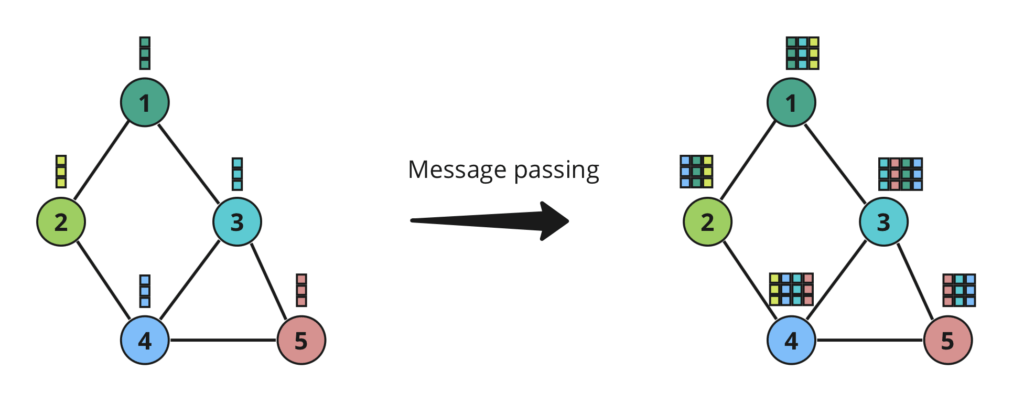
\includegraphics[width=\textwidth]{img/message_passing.png}
    \caption[Message passing]{Node features passed along edges. Reprinted from \cite{ali2023gnns}.}
    \label{fig:message_passing}
\end{figure}


\section{Boolean Satisfiability Problem}
\label{sec:SAT}
We define SAT according to Guo et al.~\cite{guo2023machine}: In propositional logic, a boolean formula is constructed from boolean variables, that only evaluate to True (1) or False (0), parentheses, and the three logic operators: conjunction ($\wedge$), disjunction ($\vee$) and negation ($\neg$). SAT aims to evaluate whether there exists a variable assignment for a formula constructed of said parts so that it evaluates to True. If so, the formula is said to be satisfiable, or unsatisfiable otherwise. 

Every propositional formula can be converted into an equivalent formula in \ac{CNF}, which consists of a conjunction of one or more clauses. These clauses are enclosed in parentheses and must contain only disjunctions of at least one literal, i.e., a variable or its negation. In this work we consider only formulae in CNF, as NeuroSAT~\cite{selsam2018learning} assumes SAT problems to be in CNF. An example of a satisfiable formula in CNF over the set of variables $V=\{x_1,x_2\}$ is 
$$\psi(V) = (x_1) \land (\neg x_1 \lor x_2) \land (\neg x_2 \lor x_2)$$
with satisfying assignment $A:\{x_1 \mapsto 1, x_2 \mapsto 1\}$. 

Furthermore, SAT is the first NP-complete problem, meaning that if there exists a deterministic algorithm able to solve SAT in polynomial time, then such an algorithm exists for every NP problem (see Cook~\cite{cook2023complexity}). Current state-of-the-art SAT solvers apply searching based methods such as Conflict Driven Clause Learning \cite{marques1999grasp} or Stochastic Local Search \cite{selman1993local} with exponential worst-case complexity.

\subsection{Representation as Bipartite Graph}
SAT has extensively been studied in the form of graphs. Guo et al.~\cite{guo2023machine} describe four different types of graph representations for CNF formulae with varying complexity and information compression. Since we want to minimize the loss of information for SAT we adapt the information-richest form of a \ac{LCG}. 
A LCG is a bipartite graph that separates literals and clauses, with edges connecting literals to the clauses they appear in (see Figure \ref{fig:lcg-sat}).
The resulting graph $G_b$ can formally be described by a biadjacency matrix $\mathbf{B}$ of shape $L \times C$, with $(L,C)$ being a bipartition of $G_b$ into literals and clauses. \\
Following Sun et al.~\cite{articleBiadjacency}, let $\mathbf{A} \in \mathbb{R}^{(L+C) \times (L+C)}$ be the adjacency matrix of our bipartite graph. Since for the bipartite case edges exist only between the two color classes $L$ and $C$, the adjacency matrix can be represented as
\begin{equation}
    \mathbf{A}(i,j) = \begin{bmatrix}
        \mathbf{0}_{L \times L} & \mathbf{B} \\
        \mathbf{B}^T & \mathbf{0}_{C \times C}
    \end{bmatrix},
\end{equation}
where $\mathbf{0}$ denotes a zero matrix in the shape of their subscript. \bigskip

\begin{figure}[h]
    \centering
    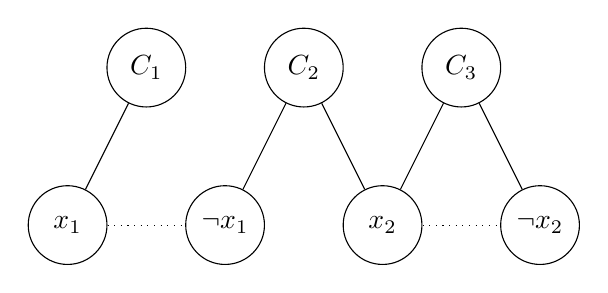
\begin{tikzpicture}[
        every node/.style={draw, circle, minimum size=1cm},
        node distance=1.5cm,
        scale=0.8,
    ]
        % Define Literal Nodes
        \node (x1) at (0, 0) {\(x_1\)};
        \node (notx1) at (2.5, 0) {\(\neg x_1\)};
        \node (x2) at (5, 0) {\(x_2\)};
        \node (notx2) at (7.5, 0) {\(\neg x_2\)};
        
        % Define Clause Nodes (one level above literals)
        \node[circle, draw] (C1) at (1.25, 2.5) {\(C_1\)};
        \node[circle, draw] (C2) at (3.75, 2.5) {\(C_2\)};
        \node[circle, draw] (C3) at (6.25, 2.5) {\(C_3\)};
        
        % Draw Edges (Literal → Clause)
        \draw (x1) -- (C1);
        \draw (notx1) -- (C2);
        \draw (x2) -- (C2);
        \draw (notx2) -- (C3);
        \draw (x2) -- (C3);
        
        % Draw Dotted Edges between each literal and its co mplement
        \draw[dotted] (x1) -- (notx1);
        \draw[dotted] (x2) -- (notx2);
    \end{tikzpicture}
    \caption[Bipartite graph in LCG]{LCG representation of $\psi(V)$ with dashed lines representing the connection between complementary literals relevant for the message passing in NeuroSAT.}
    \label{fig:lcg-sat}
\end{figure}

%\subsection{Incidence/Levi graph?}
%Defined in ALYAHYA et al. Concrete graphical representation of SAT? Type of bipartite graph.
%Defines edges via edge weight function! PART OF GRAPH THEORY \\
%Definition in Cimatti et al. : For clause $c$ we use $lit(c)$ and $var(c)$ to reference the %set of literals and variables in $c$ respectively. "$For a CNF formula F we write
%cla(F) for its set of clauses, lit(F)= c \in cla(F) lit(c) for its set of literals, and
%var(F)= c \in cla(F) var(c) for its set of variables.$"  Incidence graph of $\psi$ is the %bipartite graph $inc(\psi) = (V,E)$ with $V=lit(\psi) \cup cla(\psi)$. Additionally for %literal $x \in lit(\psi)$ and clause $c \in cla(\psi)$ we define $xc \in E$ if $x \in var(c)$.

\subsection{Unsatisfiable Cores}
The core of an unsatisfiable formula in CNF is a subset of the boolean clauses defining the formula that is also unsatisfiable. Every unsatisfiable formula therefore is a core on its own, but can be broken down into smaller cores. The smaller a core the more significance it holds \cite{10.1007/978-3-540-68237-0_23}. 

A minimal unsatisfiable core, also referred to as a \ac{MUS}, is a unsatisfiable core that becomes satisfiable whenever one of its clauses is removed \cite{dershowitz2006scalable}. It is notable that unsatisfiable SAT formulae can contain multiple MUSes, meaning that an individual MUS may be a local minimum, but not necessarily a global one \cite{liffiton2008algorithms}. SAT solvers like MiniSat~\cite{een2003extensible} are able to compute unsatisfiable cores but do not generally provide a MUS due to high computational cost. However, several deletion-based algorithms exist for computing MUSes (see Torlak et al.~\cite{10.1007/978-3-540-68237-0_23}).